\documentclass{article}
\usepackage{amsmath}
\usepackage[utf8]{inputenc}
\usepackage{graphicx} % Comandos para manejar imágenes
\graphicspath{ {./images/} } % Carpeta de imágenes
\usepackage[table,xcdraw]{xcolor}
\setlength{\parskip}{2mm} % Espaciado

\usepackage[utf8]{inputenc}
\usepackage{geometry}
    \geometry{left=3cm,right=2cm,top=2cm,bottom=2cm}
%
\usepackage[spanish]{babel}
%
\usepackage[fixlanguage]{babelbib}
    \bibliographystyle{babunsrt}
%

\usepackage{floatrow}
\floatsetup[table]{style=plaintop}

\usepackage{url}

\usepackage[top=2cm, bottom=2.5cm, right=3 cm, left=3 cm]{geometry} % margenes

\usepackage{parskip} % Sangria

\title{Seminario ocho: Eficiencia y Calidad de Vida en las comunas chilenas: comentarios sobre la presentación del Doctor Hanns De La Fuente}
\author{Cristóbal Galleguillos Ketterer$^{1}$\\
\small{$^{1}$Industrial PhD Program}\\
\small{Pontificia Universidad Católica de Valparaíso}\\
\small{cristobal.galleguillos@pucv.cl}
}
\date{\small{\today}}

\begin{document}

\maketitle

\section{Introducción}

La adopción de políticas públicas requiere necesariamente de información que permita que la asignación de recursos sea adecuada a las necesidades de la población. En muchos casos se definen parámetros cuantitativos o cualitativos que permiten que esta asignación mejore las condiciones de vida.

La calidad de vida (QoL) es un concepto general que agrupa diversas dimensiones materiales (acceso a bienes, espacios públicos), inmateriales (satisfacción, autorrealización) o de servicios (acceso a salud, educación, seguridad pública).

Al ser un concepto tan general, es necesario desarrollar modelos que permita discernir que parámetros son estadísticamente significativos para el desarrollo de estos. La eficacia de estos modelos permitirá al tomador de decisiones (en este caso el poder central) contar con la información adecuada para la asignación de recursos.
En este informe se tratará la primera de las intervenciones del doctor De La Fuente. 


\section{Revisión de la literatura}

Se realizó una revisión bibliográfica sobre el tópico, \textit{Quality of Life (QoL) in developing countries}, como este ítem es muy utilizado en ciencias de la salud, se limitó a nuestras ´pareas de interés mediante la siguiente búsqueda:

TITLE-ABS-KEY ( qol  AND developing  AND countries )  AND  ( LIMIT-TO ( SUBJAREA ,  "SOCI" )  OR  LIMIT-TO ( SUBJAREA ,  "ENVI" )  OR  LIMIT-TO ( SUBJAREA ,  "BUSI" ) )  AND  ( LIMIT-TO ( SUBJAREA ,  "ENGI" )  OR  LIMIT-TO ( SUBJAREA ,  "ECON" )  OR  LIMIT-TO ( SUBJAREA ,  "COMP" ) )

El primer hallazgo importante es la cantidad de investigaciones en este sub tópico es baja en cantidad y además se concentra en determinados países, la muestra no presenta, bajo este análisis, estudios realizados en países de Latinoamérica (Figura \ref{mapa1}.).

\begin{figure}[H]
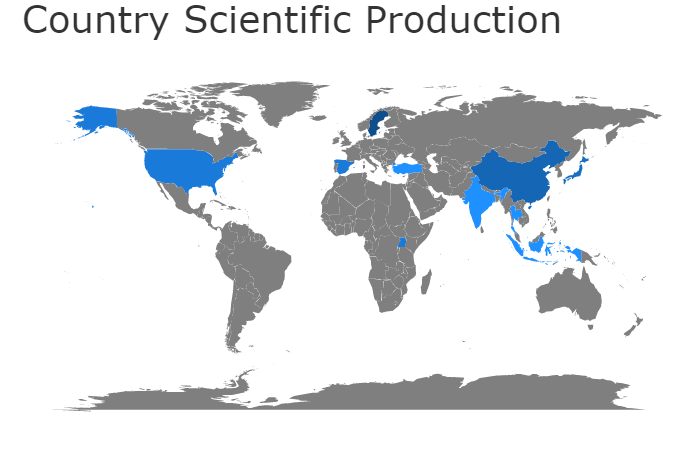
\includegraphics[scale=0.45]{Images/newplot.png}
\centering
\caption{Mapa de trabajos QoL}
\label{mapa1}
\end{figure}

Las palabras más utilizadas en los estudios de QoL se presentan en la Figura \ref{mapa2}.

\begin{figure}[H]
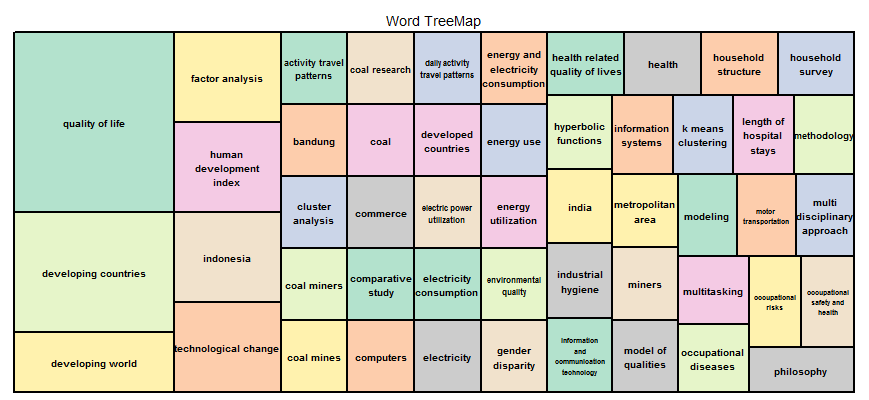
\includegraphics[scale=0.45]{Images/Mapa.png}
\centering
\caption{Mapa de palabras QoL}
\label{mapa2}
\end{figure}

\section{Marco teórico}

Calidad de Vida (QoL) es un concepto ampliamente utilizado en todos los campos del conocimiento, incluyendo a las ciencias humanas, las ciencias de la salud, las ciencias sociales y las ciencias de la ingeniería.

Como se mencionó en la introducción es un concepto muy amplio del que, a su vez, y de acuerdo a las distintas investigaciones y ramas del conocimiento, se desprenden otros conceptos.

Básicamente, la calidad de vida, se establece como una seré de parámetros e indicadores que pueden determinar una escala relativa donde podemos ubicar cierto objeto de estudio (un país, una ciudad, un grupo específico de la población) en base a estos indicadores (o un mix de estos).

Un indicador del índice de calidad de vida utilizado en Chile es el preparado por la Pontificia Universidad Católica de Santiago (PUC), los aspectos a medir en ella se presentan en la Figura \ref{UC}.

\begin{figure}[H]
\includegraphics[scale=0.45]{Images/uc.jpg}
\centering
\caption{Conceptos PUC}
\label{UC}
\end{figure}


\section{Contribución del autor}

El trabajo del profesor de la Fuente considera la representación modelos sobre calidad de vida  utilizando datos socio demográficos, estos moderan soluciones en problemas de asignación de recursos
Para el desarrollo de estos modelos se requiere el uso de econometría, por lo que la una de las líneas de investigación del profesor De La Fuente es la resolución de problemas sociales a través de métodos cuantitativos.

El trabajo presentado se basa en buscar la eficiencia de las municipalidades, que es una forma de descentralización del gobierno local, con algún margen ejecutivo.

La propuesta de este equipo es la de medir cuantificar y modelar la calidad de vista de las personas y a partir de esto definir la eficiencia de los municipios.

La hipótesis planteada se presenta a continuación (Figura \ref{hip}):

\begin{figure}[H]
\includegraphics[scale=0.45]{Images/HIPO.jpg}
\centering
\caption{Hipótesis de trabajo, Fuente \cite{article1}}
\label{hip}
\end{figure}


Para definir esta eficiencia es importante determinar qué factores se analizarán, y en base a esos considerar el impacto de dichos factores, tomando métodos estadísticos y econométricos (test “f” o el valor de $r^{2}$)

Este análisis permitió generar un pool de datos que era significativamente relevantes a la hora de medir la calidad de vida, con ellos y utilizando modelos de Cobb-Douglas y Translogaritmicos, se desarrolla una propuesta que modela matemáticamente la eficiecia de las diferentes comunas, pudiendo establecer un ranking. La eficiencia promedio de las comunas chilenas es de un 40,7 por ciento, la gráfica ((Figura \ref{ran})) presenta el resultado final del trabajo.

\begin{figure}[H]
\includegraphics[scale=0.45]{Images/rank.jpg}
\centering
\caption{Ranking de eficiencia comunas, Fuente \cite{article1}}
\label{ran}
\end{figure}


Las conclusiones del trabajo del profesor De La fuente permiten estimar que factores inciden en la eficiencia de las municipalidades (Figura \ref{q}), esto es de gran importancia por el valor que están tomando los gobiernos locales en la actualidad, la correcta asignación de recursos, y finalmente la calidad de vida de las personas.

\begin{figure}[H]
\includegraphics[scale=0.45]{Images/QOL.jpg}
\centering
\caption{Factores que afectan la calidad de vida (Qol), Fuente \cite{article1}}
\label{q}
\end{figure}

\section{Comentarios}

El trabajo del profesor De La Fuente, resulta muy interesante, ya que, a partir de datos de la realidad, se generan modelos econométricos, que permiten dar respuesta a problemáticas de tipo social.

Para medir el impacto de las políticas públicas, estos esfuerzos, son muy importantes, y demuestran que la academia puede (y debe) tener la capacidad de opinar e influir en el debate público, sobre todo en el de asignación de recursos.

La economía del bienestar está muy lejos de ser una ciencia exacta, quizás como tal, es una ciencia social que usa elementos de las matemáticas para hacer aproximaciones a la realidad. Esta más que una propuesta es una duda, en este caso de investigación, ¿Qué tanto de política y opinión debe tener la investigación? ¿Cómo la academia y el investigador, se integra como un actor político más, más allá incluso de la publicación en revistas especializadas?

Es muy probable que cuando se elige un tema de investigación o se elige tal o cual factor para analizar se está opinando, indirectamente, y hay una postura. ¿El investigador debe ser imparcial políticamente, en el texto mismo de su investigación?
\nocite{*}
    \bibliography{src/ref}

\end{document}
